\documentclass{beamer}\usepackage[]{graphicx}\usepackage[]{color}
%% maxwidth is the original width if it is less than linewidth
%% otherwise use linewidth (to make sure the graphics do not exceed the margin)
\makeatletter
\def\maxwidth{ %
  \ifdim\Gin@nat@width>\linewidth
    \linewidth
  \else
    \Gin@nat@width
  \fi
}
\makeatother

\definecolor{fgcolor}{rgb}{0.196, 0.196, 0.196}
\newcommand{\hlnum}[1]{\textcolor[rgb]{0.063,0.58,0.627}{#1}}%
\newcommand{\hlstr}[1]{\textcolor[rgb]{0.063,0.58,0.627}{#1}}%
\newcommand{\hlcom}[1]{\textcolor[rgb]{0.588,0.588,0.588}{#1}}%
\newcommand{\hlopt}[1]{\textcolor[rgb]{0.196,0.196,0.196}{#1}}%
\newcommand{\hlstd}[1]{\textcolor[rgb]{0.196,0.196,0.196}{#1}}%
\newcommand{\hlkwa}[1]{\textcolor[rgb]{0.231,0.416,0.784}{#1}}%
\newcommand{\hlkwb}[1]{\textcolor[rgb]{0.627,0,0.314}{#1}}%
\newcommand{\hlkwc}[1]{\textcolor[rgb]{0,0.631,0.314}{#1}}%
\newcommand{\hlkwd}[1]{\textcolor[rgb]{0.78,0.227,0.412}{#1}}%
\let\hlipl\hlkwb

\usepackage{framed}
\makeatletter
\newenvironment{kframe}{%
 \def\at@end@of@kframe{}%
 \ifinner\ifhmode%
  \def\at@end@of@kframe{\end{minipage}}%
  \begin{minipage}{\columnwidth}%
 \fi\fi%
 \def\FrameCommand##1{\hskip\@totalleftmargin \hskip-\fboxsep
 \colorbox{shadecolor}{##1}\hskip-\fboxsep
     % There is no \\@totalrightmargin, so:
     \hskip-\linewidth \hskip-\@totalleftmargin \hskip\columnwidth}%
 \MakeFramed {\advance\hsize-\width
   \@totalleftmargin\z@ \linewidth\hsize
   \@setminipage}}%
 {\par\unskip\endMakeFramed%
 \at@end@of@kframe}
\makeatother

\definecolor{shadecolor}{rgb}{.97, .97, .97}
\definecolor{messagecolor}{rgb}{0, 0, 0}
\definecolor{warningcolor}{rgb}{1, 0, 1}
\definecolor{errorcolor}{rgb}{1, 0, 0}
\newenvironment{knitrout}{}{} % an empty environment to be redefined in TeX

\usepackage{alltt}

% load packages
\usepackage{tikz}
\usepackage{graphicx}
\usepackage{upquote}
\usepackage{listings}
\usepackage{hyperref}
\usepackage{color}
\usepackage{lmodern}



% define a bunch of colors
\definecolor{gray}{RGB}{110,110,110}
\definecolor{darkgray}{RGB}{100,100,100}
\definecolor{lightgray}{RGB}{200,200,200}
\definecolor{lightgrey}{RGB}{200,200,200}
\definecolor{turquoise}{RGB}{81,193,188}
\definecolor{mamey}{RGB}{255,107,107}
\definecolor{tomato}{RGB}{255,136,136}
\definecolor{mandarina}{RGB}{229,169,25}
\definecolor{lemon}{rgb}{0.81,0.95,0.29}
\definecolor{bluesky}{rgb}{0.71,0.81,0.96}
\definecolor{chiclamino}{RGB}{107,174,214}
\definecolor{violet}{RGB}{133,135,211}

\definecolor{foreground}{RGB}{81,141,193}
\definecolor{background}{RGB}{246,244,240}
\definecolor{highlight}{RGB}{229,169,25}
\definecolor{lowlight}{RGB}{200,200,200}

% setting beamer colors
\setbeamercolor{title}{fg=lightgray}
\setbeamercolor{frametitle}{fg=lightgray}
\setbeamercolor{block title}{fg=turquoise}
\setbeamercolor{structure}{fg=turquoise}
\setbeamercolor{titlelike}{fg=title}
\setbeamercolor{subtitle}{fg=turquoise}
\setbeamercolor{institute}{fg=gray}
\setbeamercolor{normal text}{fg=gray,bg=background}

\setbeamercolor{palette primary}{fg=lightgray}
\setbeamercolor{palette secondary}{fg=lightgray}
\setbeamercolor{palette tertiary}{fg=lightgray}

\setbeamerfont{itemize/enumerate subbody}{size=\footnotesize}
\setbeamerfont{itemize/enumerate subitem}{size=\footnotesize}

\hypersetup{
  colorlinks=true,
  urlcolor=tomato,
  linkcolor=lightgray
}

% commands
\newcommand{\code}[1]{\texttt{#1}}
\newcommand{\high}[1]{\textcolor{highlight}{#1}}
\newcommand{\low}[1]{\textcolor{lowlight}{#1}}
\newcommand{\highcode}[1]{\textcolor{highlight}{\texttt{#1}}}


%\usecolortheme{rose}
\setbeamertemplate{blocks}[rounded]
\setbeamertemplate{footline}[frame number] 
\setbeamertemplate{navigation symbols}{}
\setbeamertemplate{frametitle}[default][center]
\useoutertheme{infolines}  % add footlines
\setbeamersize{text margin left=25pt,text margin right=25pt}



% to remove empty brackets of \institution
\makeatletter
\setbeamertemplate{footline}
{
  \leavevmode%
  \hbox{%
  \begin{beamercolorbox}[wd=.333333\paperwidth,ht=2.25ex,dp=1ex,center]{author in head/foot}%
    \usebeamerfont{author in head/foot}\insertshortauthor%~~\beamer@ifempty{\insertshortinstitute}{}{(\insertshortinstitute)}
  \end{beamercolorbox}%
  \begin{beamercolorbox}[wd=.333333\paperwidth,ht=2.25ex,dp=1ex,center]{title in head/foot}%
    \usebeamerfont{title in head/foot}\insertshorttitle
  \end{beamercolorbox}%
  \begin{beamercolorbox}[wd=.333333\paperwidth,ht=2.25ex,dp=1ex,right]{date in head/foot}%
    \usebeamerfont{date in head/foot}\insertshortdate{}\hspace*{2em}
    \insertframenumber{} / \inserttotalframenumber\hspace*{2ex} 
  \end{beamercolorbox}}%
  \vskip0pt%
}
\makeatother



\title[Getting data from the web with R]{\LARGE Getting Data from the Web with R} 
\subtitle[Web Data in R]{\large Part 6: HTTP Basics and the RCurl Package}
\author[gastonsanchez.com]{
 \textcolor{gray}{\textbf{G}aston \textbf{S}anchez}
}
\institute[]{\scriptsize \textcolor{lightgray}{April-May 2014}}
\date[CC BY-SA-NC 4.0]{
 \textcolor{lightgray}{\tiny{Content licensed under 
 \href{http://creativecommons.org/licenses/by-nc-sa/4.0/}{CC BY-NC-SA 4.0}}}
}
\IfFileExists{upquote.sty}{\usepackage{upquote}}{}
\begin{document}




%--- the titlepage frame -------------------------%

\begin{frame}[plain]
 \titlepage
\end{frame}

%------------------------------------------------

{ % all template changes are local to this group.
    \setbeamertemplate{navigation symbols}{}
    \begin{frame}[plain]
        \begin{tikzpicture}[remember picture,overlay]
            \node[at=(current page.center)] {
                
\includegraphics[width=\paperwidth]{images/http_cover.png}
            };
        \end{tikzpicture}
     \end{frame}
}

%------------------------------------------------

\begin{frame}[fragile]
\frametitle{Readme}

\begin{block}{\scriptsize License:}
\tiny
 \begin{itemize}
  \item[] Creative Commons Attribution-NonCommercial-ShareAlike 4.0 International License \\ 
  \url{http://creativecommons.org/licenses/by-nc-sa/4.0/}{}
 \end{itemize}
\end{block}

\begin{block}{\scriptsize You are free to:}
\tiny
 \begin{itemize}
  \item[] \textcolor{darkgray}{\textbf{Share}} --- \textcolor{gray}{copy and redistribute the material}
  \item[] \textcolor{darkgray}{\textbf{Adapt}} --- \textcolor{gray}{rebuild and transform the material}
 \end{itemize}
\end{block}

\vspace{2mm}
\begin{block}{\scriptsize Under the following conditions:}
\tiny
\begin{itemize}
 \item[] \textcolor{darkgray}{\textbf{Attribution}} --- \textcolor{gray}{You must give appropriate credit, provide a link to the license, and indicate if changes were made.}
 \item[] \textcolor{darkgray}{\textbf{NonCommercial}} --- \textcolor{gray}{You may not use this work for commercial purposes.}
 \item[] \textcolor{darkgray}{\textbf{Share Alike}} --- \textcolor{gray}{If you remix, transform, or build upon this 
 work, you must distribute your contributions under the same license to this one.}
\end{itemize}
\end{block}

\end{frame}

%------------------------------------------------

\begin{frame}
\frametitle{Lectures Menu}

\begin{columns}[t]
\begin{column}{0.1\textwidth}
%--- empty space ---%
\end{column}
\begin{column}{0.8\textwidth}
 \begin{block}{Slide Decks}
  \begin{enumerate}
   \item \textcolor{lightgray}{Introduction}
   \item \textcolor{lightgray}{Reading files from the Web}
   \item \textcolor{lightgray}{Basics of XML and HTML}
   \item \textcolor{lightgray}{Parsing XML / HTML content}
   \item \textcolor{lightgray}{Handling JSON data}
   \item \textbf{HTTP basics and the RCurl package}
   \item \textcolor{lightgray}{Getting data via Web forms}
   \item \textcolor{lightgray}{Getting data via Web services}
   %\item \textcolor{lightgray}{Web Scraping Case Study}
  \end{enumerate}
 \end{block}
\end{column}
\begin{column}{0.1\textwidth}
%--- empty space ---%
\end{column}
\end{columns}

\end{frame}

%------------------------------------------------

\begin{frame}
 \begin{center}
  \Huge{\textcolor{mandarina}{Web Basics}}
 \end{center}
\end{frame}

%------------------------------------------------

\begin{frame}
\frametitle{Goal}

\begin{columns}[t]
\begin{column}{0.1\textwidth}
%--- empty space ---%
\end{column}
\begin{column}{0.8\textwidth}

\begin{block}{HTTP and RCurl}
The goal of the present slides is to give you a \textbf{crash introduction to HTTP and the RCurl package} so you can be prepared to work with Web Forms (next slides)
\end{block}

\end{column}
\begin{column}{0.1\textwidth}
%--- empty space ---%
\end{column}
\end{columns}

\end{frame}

%------------------------------------------------

\begin{frame}
\frametitle{Synopsis}

\begin{columns}[t]
\begin{column}{0.1\textwidth}
%--- empty space ---%
\end{column}
\begin{column}{0.8\textwidth}

\begin{block}{In a nutshell}
We'll cover the following topics:
\begin{itemize}
 \item HTTP basics
 \item HTTP requests and responses
 \item R package \code{"RCurl"}
\end{itemize}
\end{block}

\end{column}
\begin{column}{0.1\textwidth}
%--- empty space ---%
\end{column}
\end{columns}

\end{frame}

%------------------------------------------------

\begin{frame}
\frametitle{Some References}

\begin{itemize}
 \item HTTP Basics tutorial \\
 {\tiny \url{http://www3.ntu.edu.sg/home/ehchua/programming/webprogramming/http_basics.html}}
 \item The RCurl Package \\
 {\scriptsize \url{http://www.omegahat.org/RCurl/}}
 \item R as a Web Client --- the RCurl Package \\
 {\scriptsize \url{http://www.omegahat.org/RCurl/RCurlJSS.pdf}}
 \item XML and Web Technlogies for Data Sciences with R \\
 \low{by Deb Nolan and Duncan Temple Lang}
 \item \code{libcurl}: the C-URL library \\
 {\scriptsize \url{http://curl.haxx.se/libcurl/}}
\end{itemize}

\end{frame}

%------------------------------------------------

\begin{frame}
\frametitle{Considerations}

\begin{columns}[t]
\begin{column}{0.1\textwidth}
%--- empty space ---%
\end{column}
\begin{column}{0.8\textwidth}

\begin{block}{Keep in mind}
We will discuss preliminary material that will help you understand how to work with data using Web (HTML) Forms:
\begin{itemize}
 \item Overview of how the Web works
 \item Basics of \textbf{HTTP requests}
 \item R package \highcode{"RCurl"}
\end{itemize}
\end{block}

\end{column}
\begin{column}{0.1\textwidth}
%--- empty space ---%
\end{column}
\end{columns}

\end{frame}

%------------------------------------------------

\begin{frame}
 \begin{center}
  \Huge{\textcolor{mandarina}{Web Basics}}
 \end{center}
\end{frame}

%------------------------------------------------

\begin{frame}
\frametitle{Surfing the Web}

\begin{center}
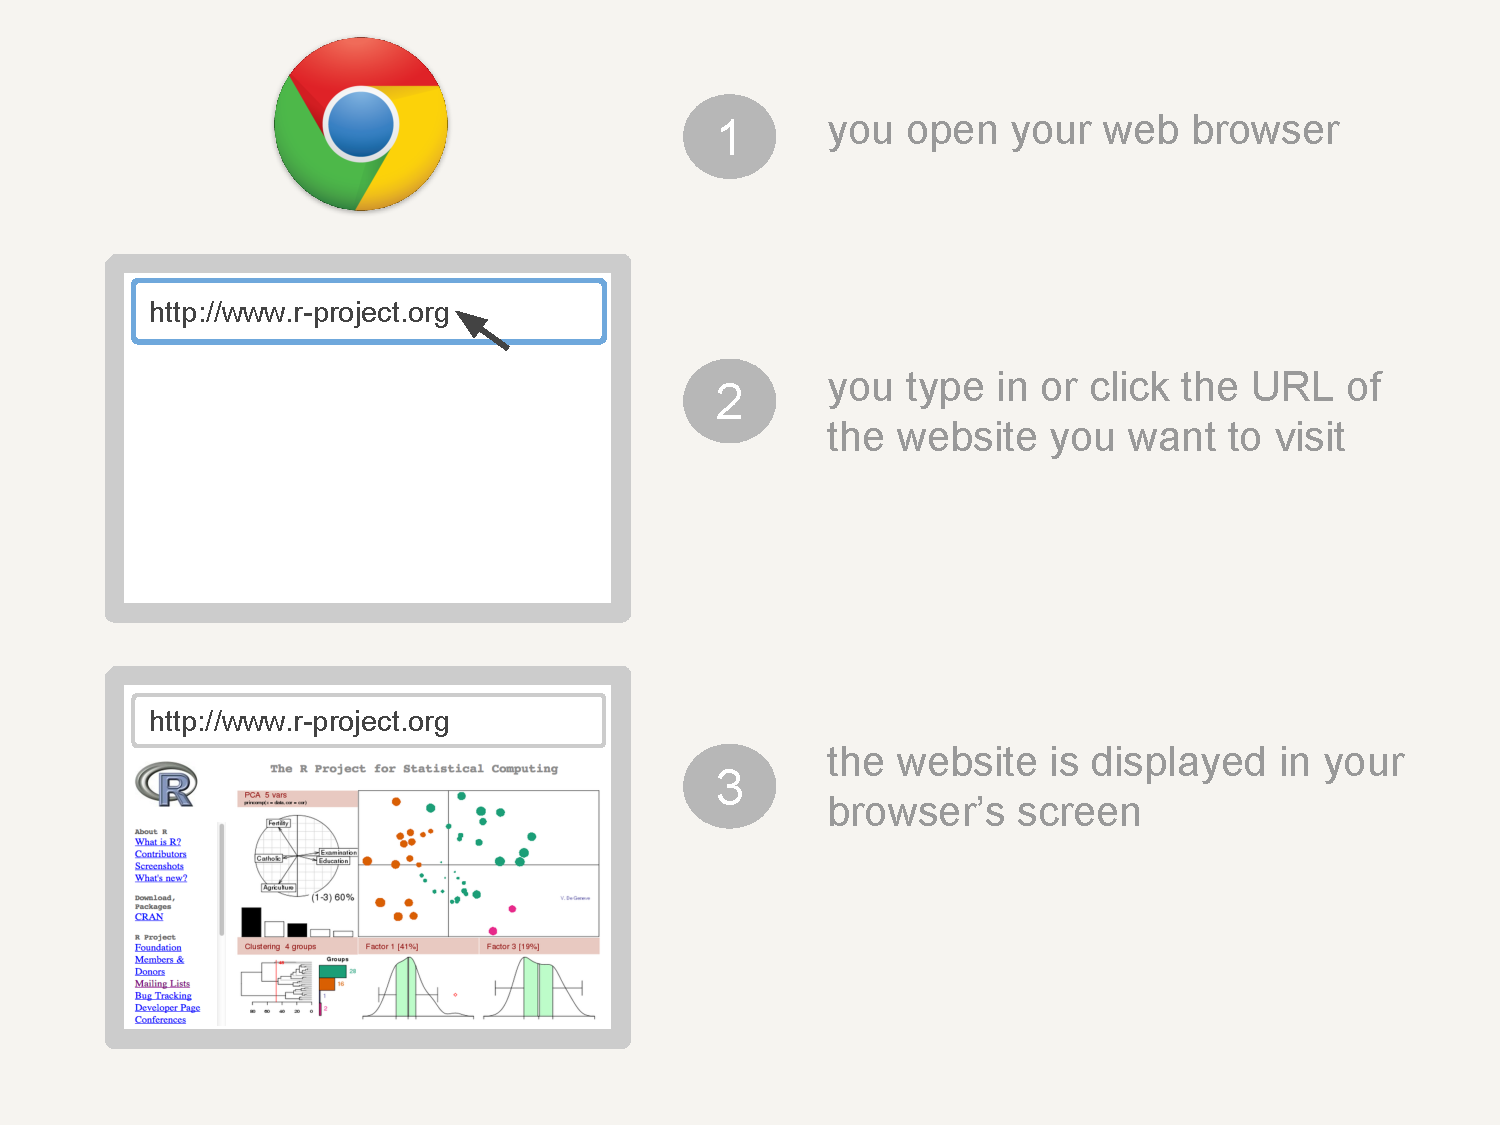
\includegraphics[width=11cm]{images/web_surfing.pdf}
\end{center}

\end{frame}

%------------------------------------------------

\begin{frame}
\frametitle{Surfing the Web}

\begin{block}{Think about when you surf the web:}
\begin{itemize}
 \item you open a browser \\
 \low{(eg chrome, mozilla, safari, internet explorer, etc)}
 \item you type in or click the URL of a website you wish to visit \\
 \low{(eg \code{http://www.r-project.org})}
 \item you wait some fractions of a second
 \item and then the website shows up in your screen
\end{itemize}
\end{block}

\end{frame}

%------------------------------------------------

\begin{frame}
\frametitle{More Formally ...}

\begin{block}{Surfing the Web}
\begin{itemize}
 \item People access websites using software called a \textbf{web browser} \\
 \low{(eg Firefox, Chrome, Safari, Internet Explorer)}
 \item The browser in your computer is the \textbf{client that requests} a variety of resources \low{(eg pages, images, video, audio, scripts)}
 \item The client's request is sent to \textbf{web servers}
 \item The server \textbf{sends responses} back to the client
 \item The way Clients and Servers dialogue between each other is by following formal \textbf{protocols of communication}
\end{itemize}
\end{block}

\end{frame}

%------------------------------------------------

\begin{frame}
\frametitle{The Web}

\begin{center}
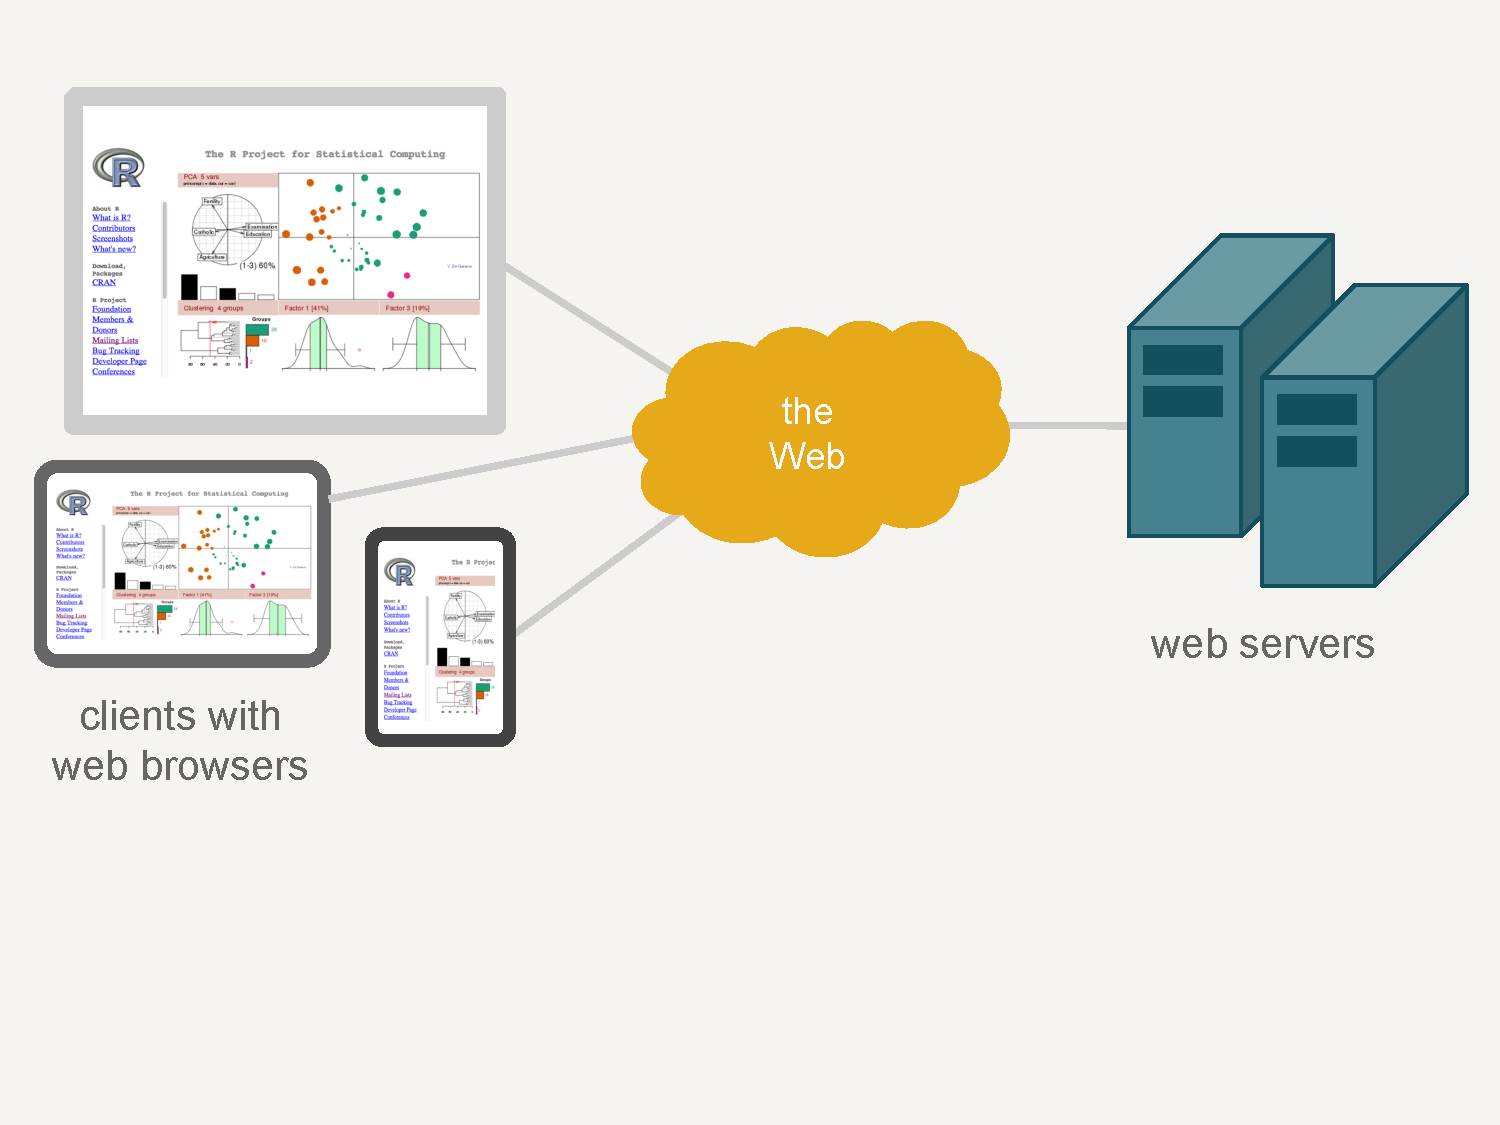
\includegraphics[width=11.5cm]{images/clients_servers.pdf}
\end{center}

\end{frame}

%------------------------------------------------

\begin{frame}
\frametitle{Basics First}

\begin{block}{About the Web}
\begin{itemize}
 \item The Web is a massive distributed information system connecting software-and-computers to share information.
 \item The software-and-computers that form the Web are divided in two types: \textit{clients} and \textit{servers}.
 \item A \textbf{client} is the software that \high{\textit{requests}} information \\
 \low{(eg html pages, scripts, images, video, audio)}
 \item A \textbf{server} is the software-computer in charge of \high{\textit{serving}} the resources that the clients request.
 \item Clients and Servers communicate via the \textbf{HyperText Transfer Protocol} (HTTP) and other protocols.
\end{itemize}
\end{block}

\end{frame}

%------------------------------------------------

\begin{frame}
 \begin{center}
  {\Huge \textcolor{mandarina}{HTTP}}
  
  \bigskip
  {\Large \textcolor{mandarina}{HyperText Transfer Protocol}}
 \end{center}
\end{frame}

%------------------------------------------------

\begin{frame}
\frametitle{Protocol}

\begin{quotation}
``\textbf{Protocol}: a system of rules that explain the correct conduct and procedures to be followed in formal situations''
\end{quotation}

{\footnotesize 
\hspace{8mm} \url{http://www.merriam-webster.com/dictionary/protocol}
}

\vspace{10mm}

\begin{quotation}
``A \textbf{communications protocol} is a system of digital rules for data exchange within or between computers''
\end{quotation}

{\footnotesize 
\hspace{8mm} \url{http://en.wikipedia.org/wiki/Communications_protocol}
}

\end{frame}

%------------------------------------------------

\begin{frame}
\frametitle{About HTTP}

\begin{block}{What is HTTP?}
\begin{itemize}
 \item HTTP stands for \textbf{HyperText Transfer Protocol}
 \item HTTP allows clients and servers to communicate \\
 \low{(send and receive messages)}
 \item HTTP can be used to transfer documents, images, movies, audio files, 
data, scripts and all the other web resources that make up websites and applications
\end{itemize}
\end{block}

\end{frame}

%------------------------------------------------

\begin{frame}
\frametitle{Surfing the Web}

\begin{center}
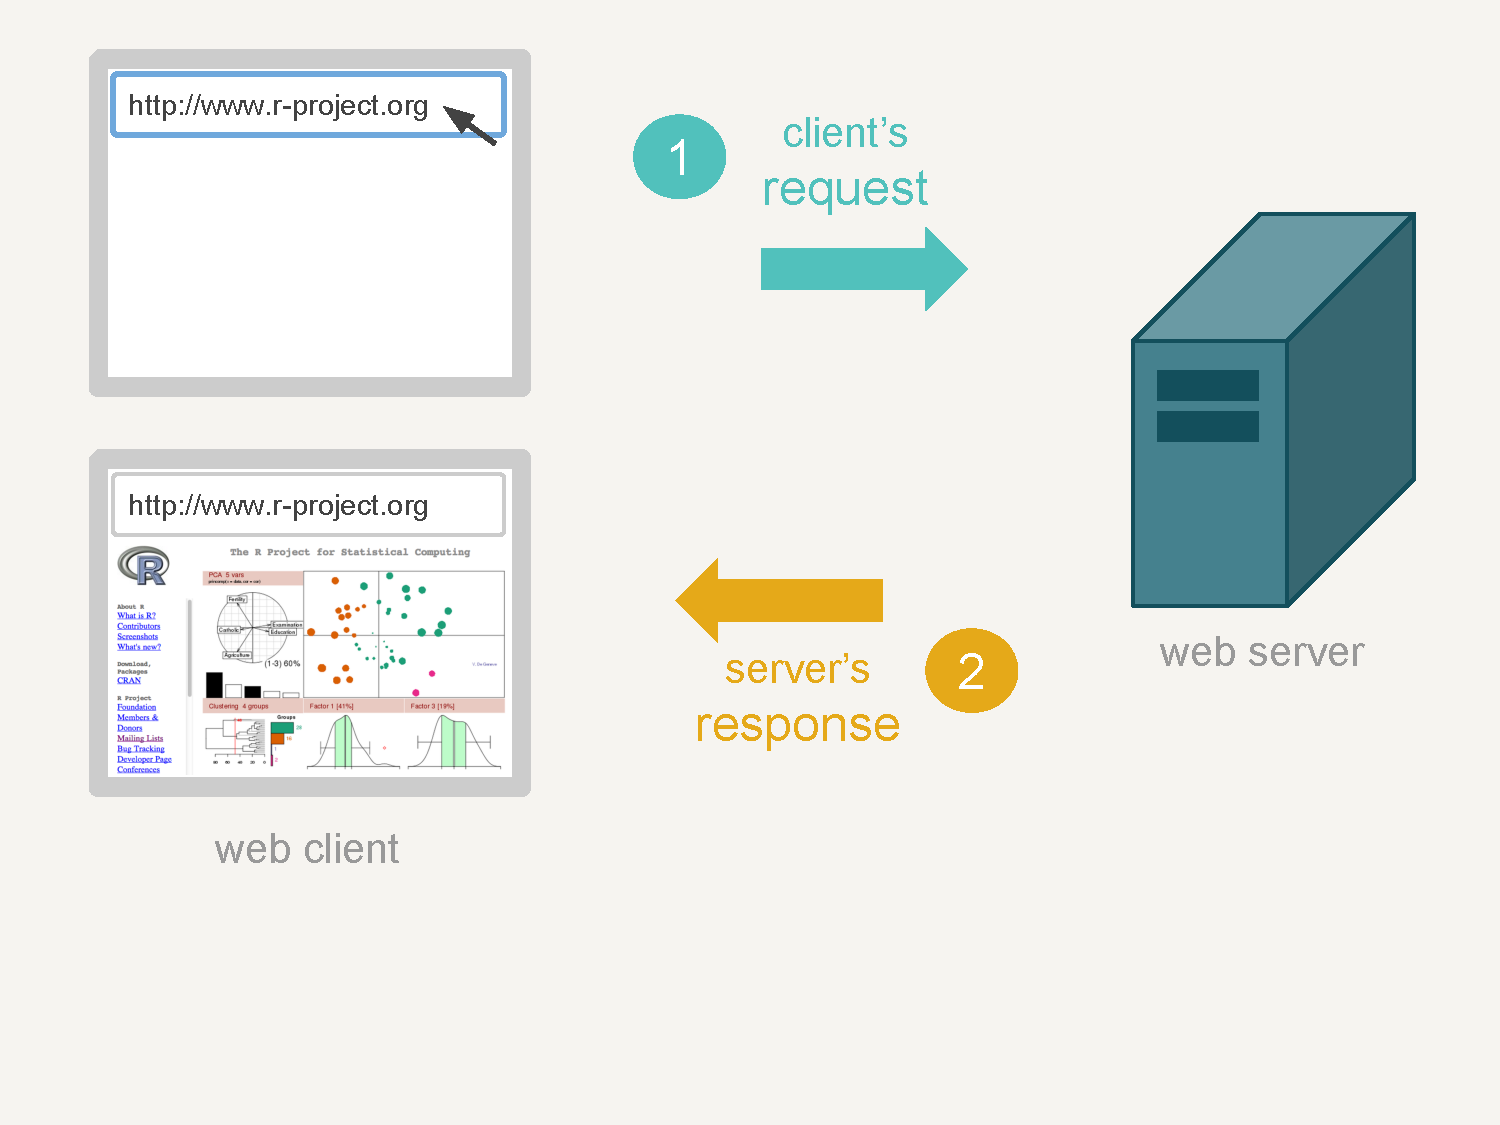
\includegraphics[width=11cm]{images/client_request_server_response.pdf}
\end{center}

\end{frame}

%------------------------------------------------

\begin{frame}
\frametitle{Behind the Scenes}

\begin{block}{Whenever you surf the web:}
\begin{itemize}
 \item your browser sends \textbf{HTTP request} messages \\
 \low{(for HTML pages, images, scripts and styles sheets)}
 \item the HTTP requests are sent to Web servers
 \item Web servers handle these requests by returning \textbf{HTTP response} messages
 \item the responses contain the requested resource
\end{itemize}
\end{block}

\end{frame}

%------------------------------------------------

\begin{frame}
\frametitle{HTTP Requests and Responses}

Suppose we open the browser in order to visit the R project's homepage

\begin{center}
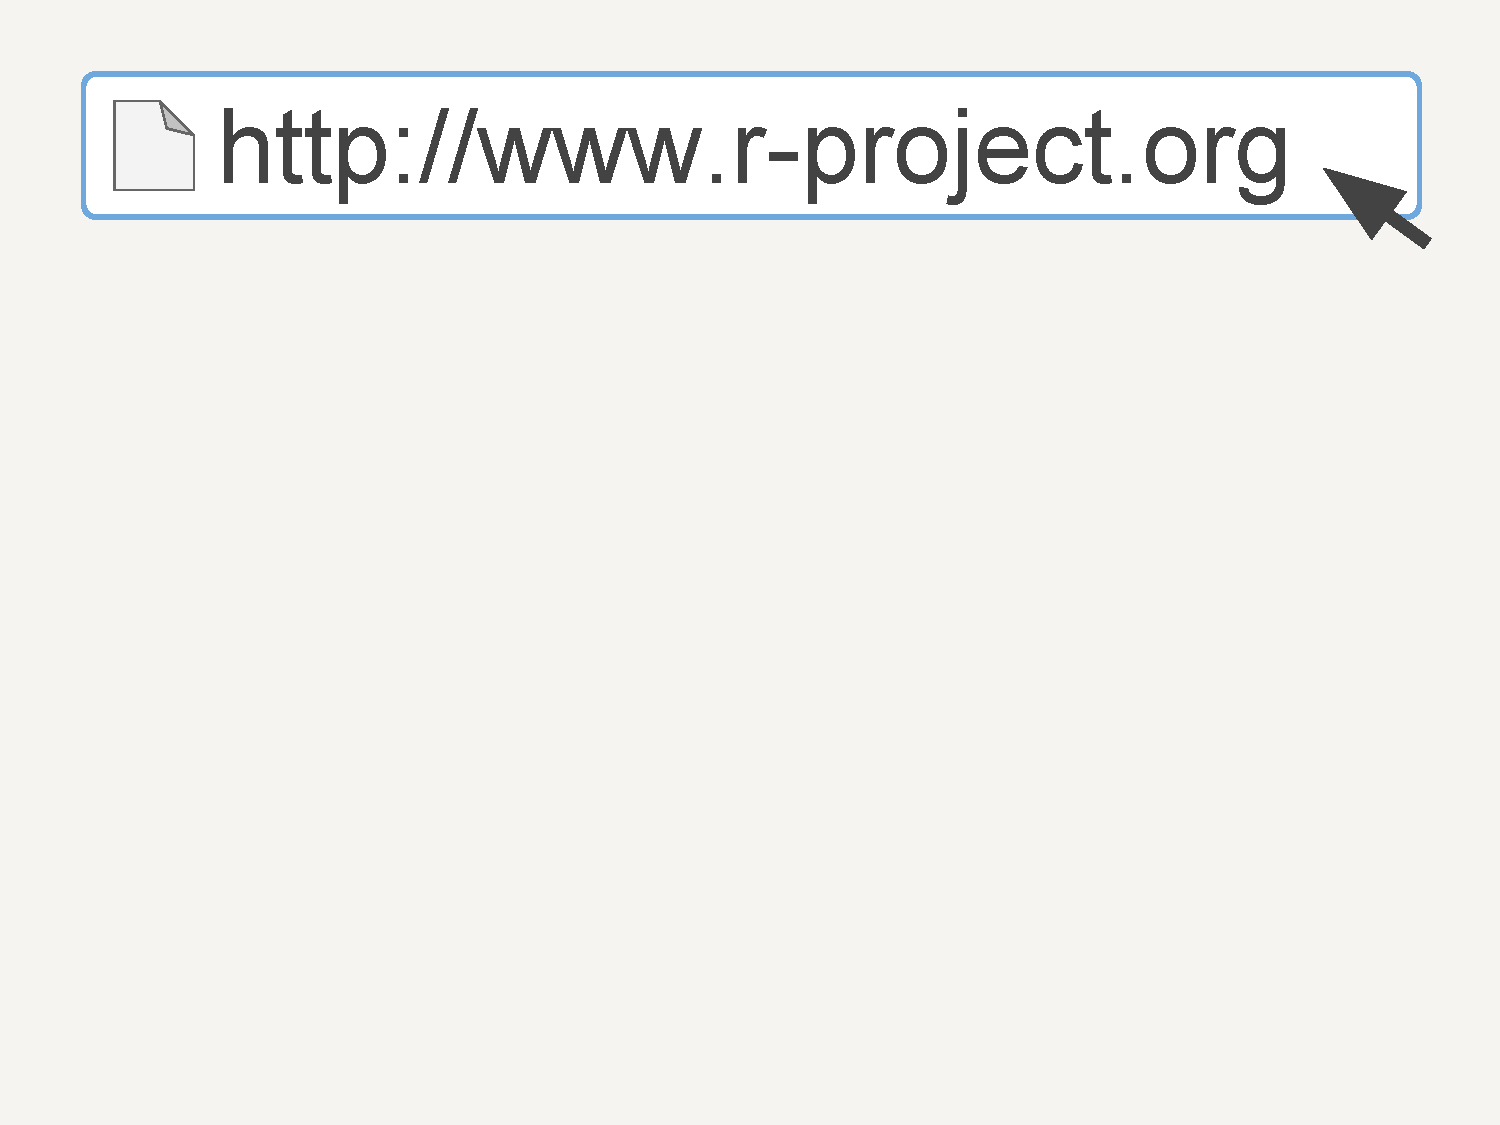
\includegraphics[width=8cm]{images/web_request.pdf}
\end{center}

\end{frame}

%------------------------------------------------

\begin{frame}[fragile]
\frametitle{HTTP Request and Response}

Although we don't see it, there's a client-server dialogue:

{\tiny
\begin{verbatim}
GET / HTTP/1.1
User-Agent: curl/7.24.0 (x86_64-apple-darwin12.0) libcurl/7.24.0 OpenSSL/0.9.8y zlib/1.2.5
Host: r-project.org
Accept: */*

-------------------------------------------------------------------------------------------

HTTP/1.1 301 Moved Permanently
Date: Thu, 01 May 2014 16:54:43 GMT
Server: Apache/2.2.22 (Debian)
Location: http://www.r-project.org/
Vary: Accept-Encoding
Content-Length: 312
Content-Type: text/html; charset=iso-8859-1
 
<!DOCTYPE HTML PUBLIC "-//IETF//DTD HTML 2.0//EN">
<html><head>
<title>301 Moved Permanently</title>
</head><body>
<h1>Moved Permanently</h1>
<p>The document has moved <a href="http://www.r-project.org/">here</a>.</p>
<hr>
<address>Apache/2.2.22 (Debian) Server at r-project.org Port 80</address>
</body></html>
\end{verbatim}
}

\end{frame}

%------------------------------------------------

\begin{frame}
\frametitle{Client HTTP Request and Server HTTP Response}

\begin{center}
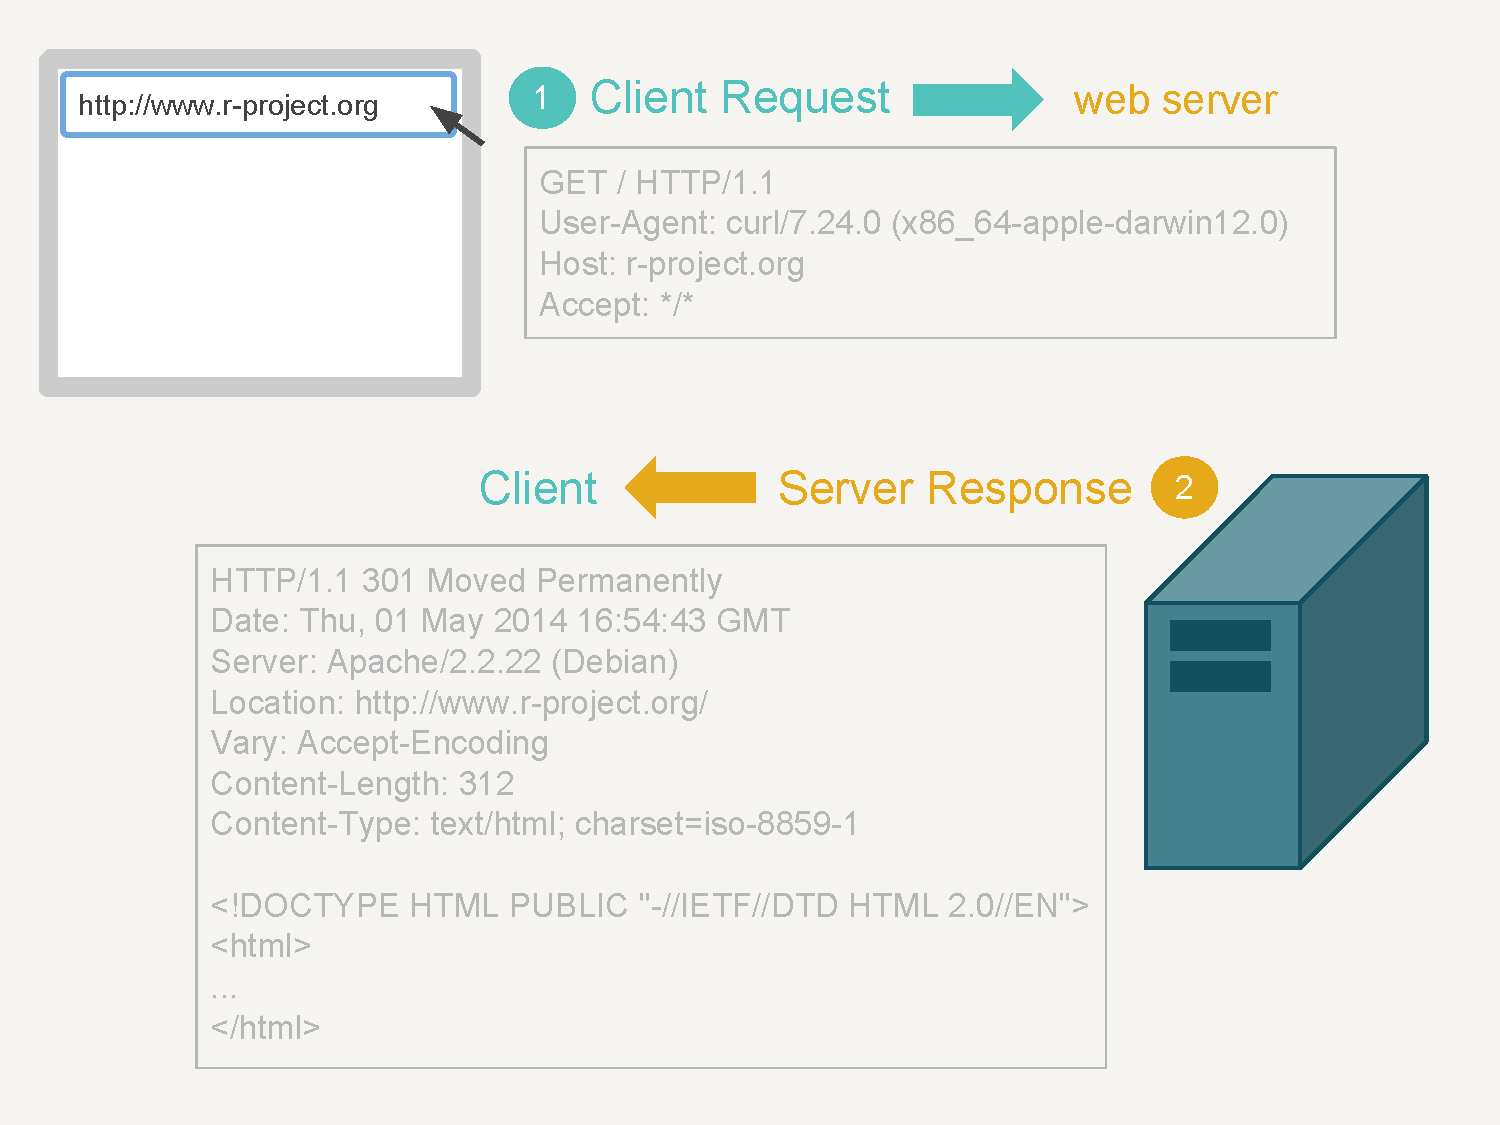
\includegraphics[width=10cm]{images/http_request_response.pdf}
\end{center}

\end{frame}

%------------------------------------------------

\begin{frame}
\frametitle{HTTP Messages}

\begin{block}{Anatomy of an HTTP message}
HTTP messages consist of 2 parts \low{(separated by a blank line)} 
\begin{enumerate}
 \item A message \textbf{header}
 \begin{itemize}
  \item the 1st line in the header is the request/response line
  \item the rest of the lines are \textit{headers} formed of \code{name:value} pairs
 \end{itemize}
 \item An optional message \textbf{body}
\end{enumerate}
\end{block}

\end{frame}

%------------------------------------------------

\begin{frame}[fragile]
\frametitle{Anatomy of an HTTP Request}

The client \low{(your browser)} sends a \textbf{request} to the server:

{\tiny
\begin{verbatim}
GET / HTTP/1.1
User-Agent: curl/7.24.0 (x86_64-apple-darwin12.0) libcurl/7.24.0 OpenSSL/0.9.8y zlib/1.2.5
Host: r-project.org
Accept: */*
\end{verbatim}
}

\begin{itemize}
 \item The first line is the \textbf{request line} which contains: \\
 {\footnotesize \code{GET / HTTP/1.1}}
 \item The rest of the \textit{headers} are just \code{name:value} pairs \\
{\footnotesize eg \code{Host: r-project.org}}
\end{itemize}

\end{frame}

%------------------------------------------------

\begin{frame}[fragile]
\frametitle{Anatomy of an HTTP Response}

The server sends a \textbf{response} to the client:

{\tiny
\begin{verbatim}
HTTP/1.1 301 Moved Permanently
Date: Thu, 01 May 2014 16:54:43 GMT
Server: Apache/2.2.22 (Debian)
Location: http://www.r-project.org/
Vary: Accept-Encoding
Content-Length: 312
Content-Type: text/html; charset=iso-8859-1
 
<!DOCTYPE HTML PUBLIC "-//IETF//DTD HTML 2.0//EN">
<html>
...
</html>
\end{verbatim}
}

\begin{itemize}
 \item The first line is the \textbf{status line} which contains: \\
 {\footnotesize \code{GET / HTTP/1.1}}
 \item The next lines contain \textbf{header values}
 \item The \textbf{body} message appears after the blank line \\
 \low{in this case is the content of the HTML page}
\end{itemize}

\end{frame}

%------------------------------------------------

\begin{frame}
 \begin{center}
  \Huge{\textcolor{mandarina}{HTTP Methods}}
 \end{center}
\end{frame}

%------------------------------------------------

\begin{frame}
\frametitle{HTTP Methods}

\begin{center}
 \begin{tabular}{l l}
  \hline
  Method & Description \\
  \hline
  \code{GET} & retrieves whatever information is identified \\
  & by the Request-URI \\
  \hline
  \code{POST} & request with data enclosed in the request body \\
  \hline
  \code{HEAD} &  identical to GET except that the server MUST NOT \\
  & return a message-body in the response \\
  \hline
  \code{PUT} & requests that the enclosed entity be stored under \\
  & the supplied Request-URI \\
  \hline
  \code{DELETE} & requests that the origin server delete the resource \\
  & identified by the Request-URI \\
  \hline
  \code{TRACE} & invokes a remote, application-layer loop-back of the \\
  & request message \\
  \hline
  \code{CONNECT} & for use with a proxy that can dynamically switch \\
  & to being a tunnel  \\
  \hline
 \end{tabular}
\end{center}

\end{frame}

%------------------------------------------------

\begin{frame}
\frametitle{Quick Recap}

\begin{block}{So far we've seen that:}
\begin{itemize}
 \item The HTTP protocol is a standardized method for transferring data or documents over the Web
 \item The clients' requests and the servers' responses are handled via the HTTP protocol
 \item There are 2 types of HTTP messages: \textbf{requests} and \textbf{responses}
 \item We don't actually see HTTP messages but they are there \textit{behind the scenes}
 \end{itemize}
\end{block}

\end{frame}

%------------------------------------------------

\begin{frame}
 \begin{center}
  \Huge{\textcolor{mandarina}{R package \code{"RCurl"}}}
 \end{center}
\end{frame}

%------------------------------------------------

\begin{frame}
\frametitle{Why RCurl?}

\begin{quotation}
``The Web is clearly an important source of data for statisticians as is emerging as vital component in distributed computing via Web services. HTTP is the primary mechanism that underlies the Web and data transfer. As such, it is important for programming languages to have tools for HTTP requests and other protocols''
\end{quotation}

{\footnotesize 
\hspace{8mm} \low{Duncan Temple Lang} \\
\hspace{8mm} \url{http://www.omegahat.org/RCurl/RCurlJSS.pdf}
}

\end{frame}

%------------------------------------------------

{ % all template changes are local to this group.
    \setbeamertemplate{navigation symbols}{}
    \begin{frame}[plain]
        \begin{tikzpicture}[remember picture,overlay]
            \node[at=(current page.center)] {
                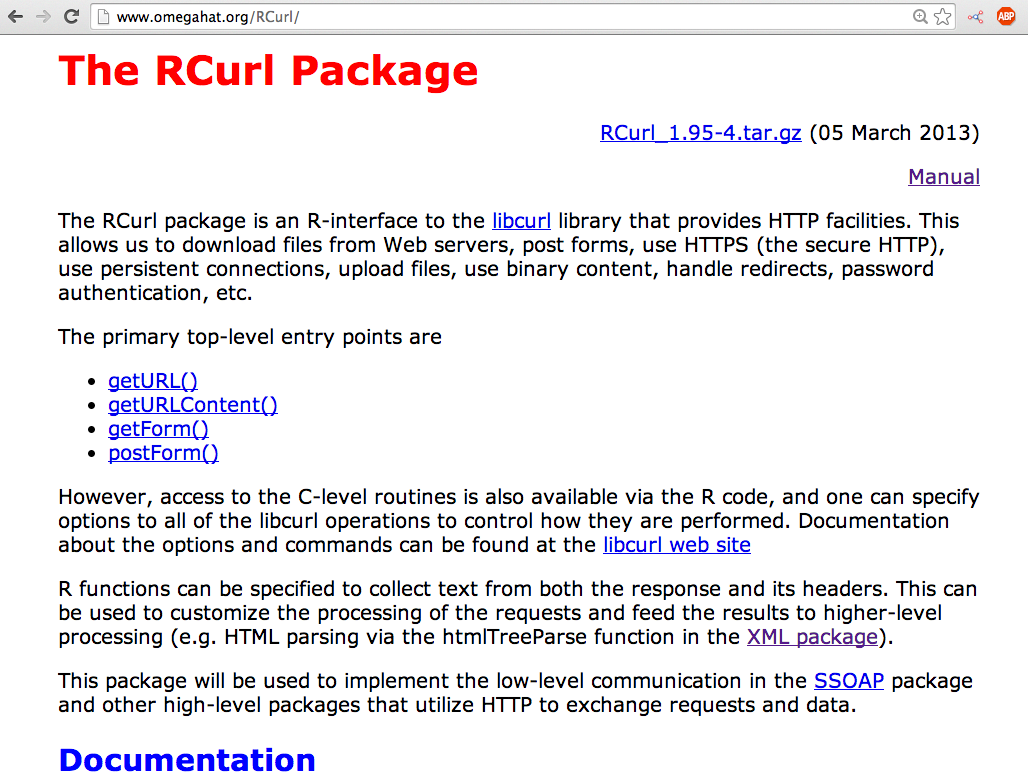
\includegraphics[width=\paperwidth]{images/rcurl_website.png}
            };
        \end{tikzpicture}
     \end{frame}
}

%------------------------------------------------

\begin{frame}
\frametitle{Package \code{"RCurl"}}

\begin{block}{RCurl}
The R package \highcode{"RCurl"} provides the necessary tools for accessing URIs, data and services via HTTP.

\bigskip

Basically, \highcode{"RCurl"} is an R-interface to the C-library \code{libcurl} \\
\low{(which provides HTTP facilities)}

\bigskip

It is developed by Duncan Temple Lang and the \textit{official} documentation is available at: \\
\url{http://www.omegahat.org/RCurl}

\end{block}

\end{frame}

%------------------------------------------------

\begin{frame}
\frametitle{About RCurl}

\begin{block}{Why RCurl?}
R has very basic ---\textit{limited}--- support for HTTP facilities. But \highcode{"RCurl"} provides \textit{steroids} to R for handling HTTP as well as other protocols.

\bigskip

Simply put, \highcode{"RCurl"} allows us to \textbf{use R as a Web Client}.
\end{block}

\end{frame}

%------------------------------------------------

\begin{frame}
\frametitle{About RCurl}

\begin{block}{RCurl}
\begin{itemize}
 \item provides an R interface to client-side HTTP
 \item is based on \textit{libcurl}: the \code{cURL} C-level library \\
{\scriptsize \url{http://curl.haxx.se/libcurl}}
 \item has support for numerous protocols \\
 \low{(eg HTTP, HTTPS, FTP, FTPS, TFTP, LDAP)}
 \item provides the infrastructure to build web-based client software
\end{itemize}
\end{block}

\end{frame}

%------------------------------------------------

\begin{frame}
\frametitle{What does RCurl do?}

\begin{block}{\code{"RCurl"} allows us to:}
\begin{itemize}
 \item download URLs 
 \item submit forms in different ways
 \item supports HTTPS \low{(the secure HTTP)}
 \item handle authentication using passwords
 \item use FTP to download files
 \item use persistent connections
 \item upload files
 \item handle escaping characters in requests
 \item handle binary data
\end{itemize}
\end{block}

\end{frame}

%------------------------------------------------

\begin{frame}
\frametitle{High-Level Functions in RCurl}

\begin{block}{High-level functions}
There are 3 high-level functions in \code{"RCurl"}: 
\end{block}

\begin{center}
 \begin{tabular}{l l}
  \hline
  Function & Description \\
  \hline
  \highcode{getURL()} & fetches the content of a URI \\
  \highcode{getForm()} & submits a Web form via the \code{GET} method  \\
  \highcode{postForm()} & submits a Web form via the \code{POST} method  \\
  \hline
 \end{tabular}
\end{center}

\end{frame}

%------------------------------------------------

\begin{frame}
\frametitle{High-Level Functions in RCurl}

\begin{block}{Main Characteristics of high-level functions}
\begin{itemize}
 \item they take a URI and other optional parameters
 \item they send an HTTP request and expect a document in response
 \item they differ in the type of document they retrieve and how
\end{itemize}
\end{block}

\end{frame}

%------------------------------------------------

\begin{frame}[fragile]
\frametitle{Function \code{getURL()}}

\begin{block}{Function \code{getURL()}}
As its name indicates, this function allows us to fetch the contents of a URL. 

\bigskip
\highcode{getURL()} expands the somewhat limited capabilities provided by the built-in functions \code{download.url()} and \code{url()}
\end{block}

\end{frame}

%------------------------------------------------

\begin{frame}[fragile]
\frametitle{Function \code{getURL()}}

\begin{block}{Using \code{getURL()}}
\code{getURL()} downloads \textit{static or fixed content} files. It collects and returns the body of the response into a single string.

\bigskip
For instance, let's fetch the content of the R-project's homepage
\end{block}

\begin{knitrout}\tiny
\definecolor{shadecolor}{rgb}{1, 1, 1}\color{fgcolor}\begin{kframe}
\begin{alltt}
\hlcom{# load RCurl (remember to install it first)}
\hlkwd{library}\hlstd{(RCurl)}

\hlcom{# retrieving the content of the R homepage}
\hlstd{Rproj} \hlkwb{=} \hlkwd{getURL}\hlstd{(}\hlstr{"http://www.r-project.org/"}\hlstd{)}
\end{alltt}
\end{kframe}
\end{knitrout}


\end{frame}

%------------------------------------------------

\begin{frame}[fragile]
\frametitle{Function \code{getURL()}}

If you inspect the content of \code{Rproj}, you should see this:

{\scriptsize
\begin{verbatim}
[1] "<!DOCTYPE HTML PUBLIC \"-//W3C//DTD HTML 4.01 Transitional//EN\">\n
<html>\n<head>\n<title>The R Project for Statistical Computing</title>\n
<link rel=\"icon\" href=\"favicon.ico\" type=\"image/x-icon\">\n<link rel
=\"shortcut icon\" href=\"favicon.ico\" type=\"image/x-icon\">\n<link rel
=\"stylesheet\" type=\"text/css\" href=\"R.css\">\n</head>\n\n<FRAMESET cols
=\"1*, 4*\" border=0>\n<FRAMESET rows=\"120, 1*\">\n<FRAME src=\"logo.html\" 
name=\"logo\" frameborder=0>\n<FRAME src=\"navbar.html\" name=\"contents\" 
frameborder=0>\n</FRAMESET>\n<FRAME src=\"main.shtml\" name=\"banner\" 
frameborder=0>\n<noframes>\n<h1>The R Project for Statistical Computing</h1
>\n\nYour browser seems not to support frames,\nhere is the <A href=\"navbar
.html\">contents page</A> of the R Project's\nwebsite.\n</noframes>\n
</FRAMESET>\n\n\n\n"
\end{verbatim}
}

\end{frame}

%------------------------------------------------

\begin{frame}[fragile]
\frametitle{Function \code{getURL()}}

\begin{block}{\code{getURL()} output}
What can we do with the retrieved content in \code{Rproj}? 

We can parse it using the functions from the \code{"XML"} package:
\end{block}

\begin{knitrout}\tiny
\definecolor{shadecolor}{rgb}{1, 1, 1}\color{fgcolor}\begin{kframe}
\begin{alltt}
\hlcom{# load XML}
\hlkwd{library}\hlstd{(XML)}

\hlcom{# parsing the content of the R homepage}
\hlstd{Rproj_doc} \hlkwb{=} \hlkwd{htmlParse}\hlstd{(Rproj)}
\end{alltt}
\end{kframe}
\end{knitrout}

\begin{knitrout}\tiny
\definecolor{shadecolor}{rgb}{1, 1, 1}\color{fgcolor}\begin{kframe}


{\ttfamily\noindent\itshape\color{messagecolor}{\#\# Loading required package: methods}}\end{kframe}
\end{knitrout}

\end{frame}

%------------------------------------------------

\begin{frame}
\frametitle{RCurl for web Forms?}

\begin{block}{\code{"RCurl"} and Web Forms}
The real power and \textit{raison d'etre} of \code{"RCurl"} is its capacity for making requests associated to Web Forms
\end{block}

\begin{block}{\code{"RCurl"} for Web Forms}
Go check the next slides!!!
\end{block}

\end{frame}

%------------------------------------------------

\end{document}
